\documentclass[12pt]{ctexbook}
\usepackage{fancyhdr,color,graphicx,CJKnumb}
\usepackage{amsfonts,anysize,amscd,amsthm,amsmath}
\marginsize{3.5cm}{2cm}{2cm}{1.5cm} % 定义页边距

\usepackage{txfonts,esint}
%选用 txfonts 数学字体,用esint换掉其丑陋的积分号

\newcommand{\chap}[1]{\chapter{#1}\fancyhead[CE]{第\CJKnumber{\thechapter}章\quad
#1}\fancyhead[CO]{\S\rightmark}}

\usepackage[colorlinks,urlcolor=blue,citecolor=blue,linkcolor=blue]{hyperref}
\hypersetup{CJKbookmarks={true}}
\newtheorem{thm}{定理}[section]
\newtheorem{cor}[thm]{推论}
\newtheorem{lem}[thm]{引理}
\newtheorem{prop}[thm]{命题}
\theoremstyle{definition}
\newtheorem{defn}[thm]{定义}
\theoremstyle{remark}
\newtheorem{rem}[thm]{注}
\newtheorem*{pf}{\CJKfamily{kai}{证}}
\newtheorem{exmp}[thm]{例}
\newtheorem{prob}[thm]{Problem}

\allowdisplaybreaks
\begin{document}
%% 使用方法:
%% 1) 在 cov.doc 中填写论文题目、作者姓名等信息
%% 2) 存盘后转为 PDF文件 cov.pdf,用于替换本目录所附的 cov.pdf。
%% 3) 然后,在本 TeX 文件中撰写学位论文的内容(用 \chap{} 开始新的一章)
%% 4) 以 pdflatex 编译,即可得到学位论文的 PDF 文件。

%%%%封面, 原创性声明, 使用说明等
\pagestyle{empty}
\vspace*{-10pt}
\hspace{-20pt}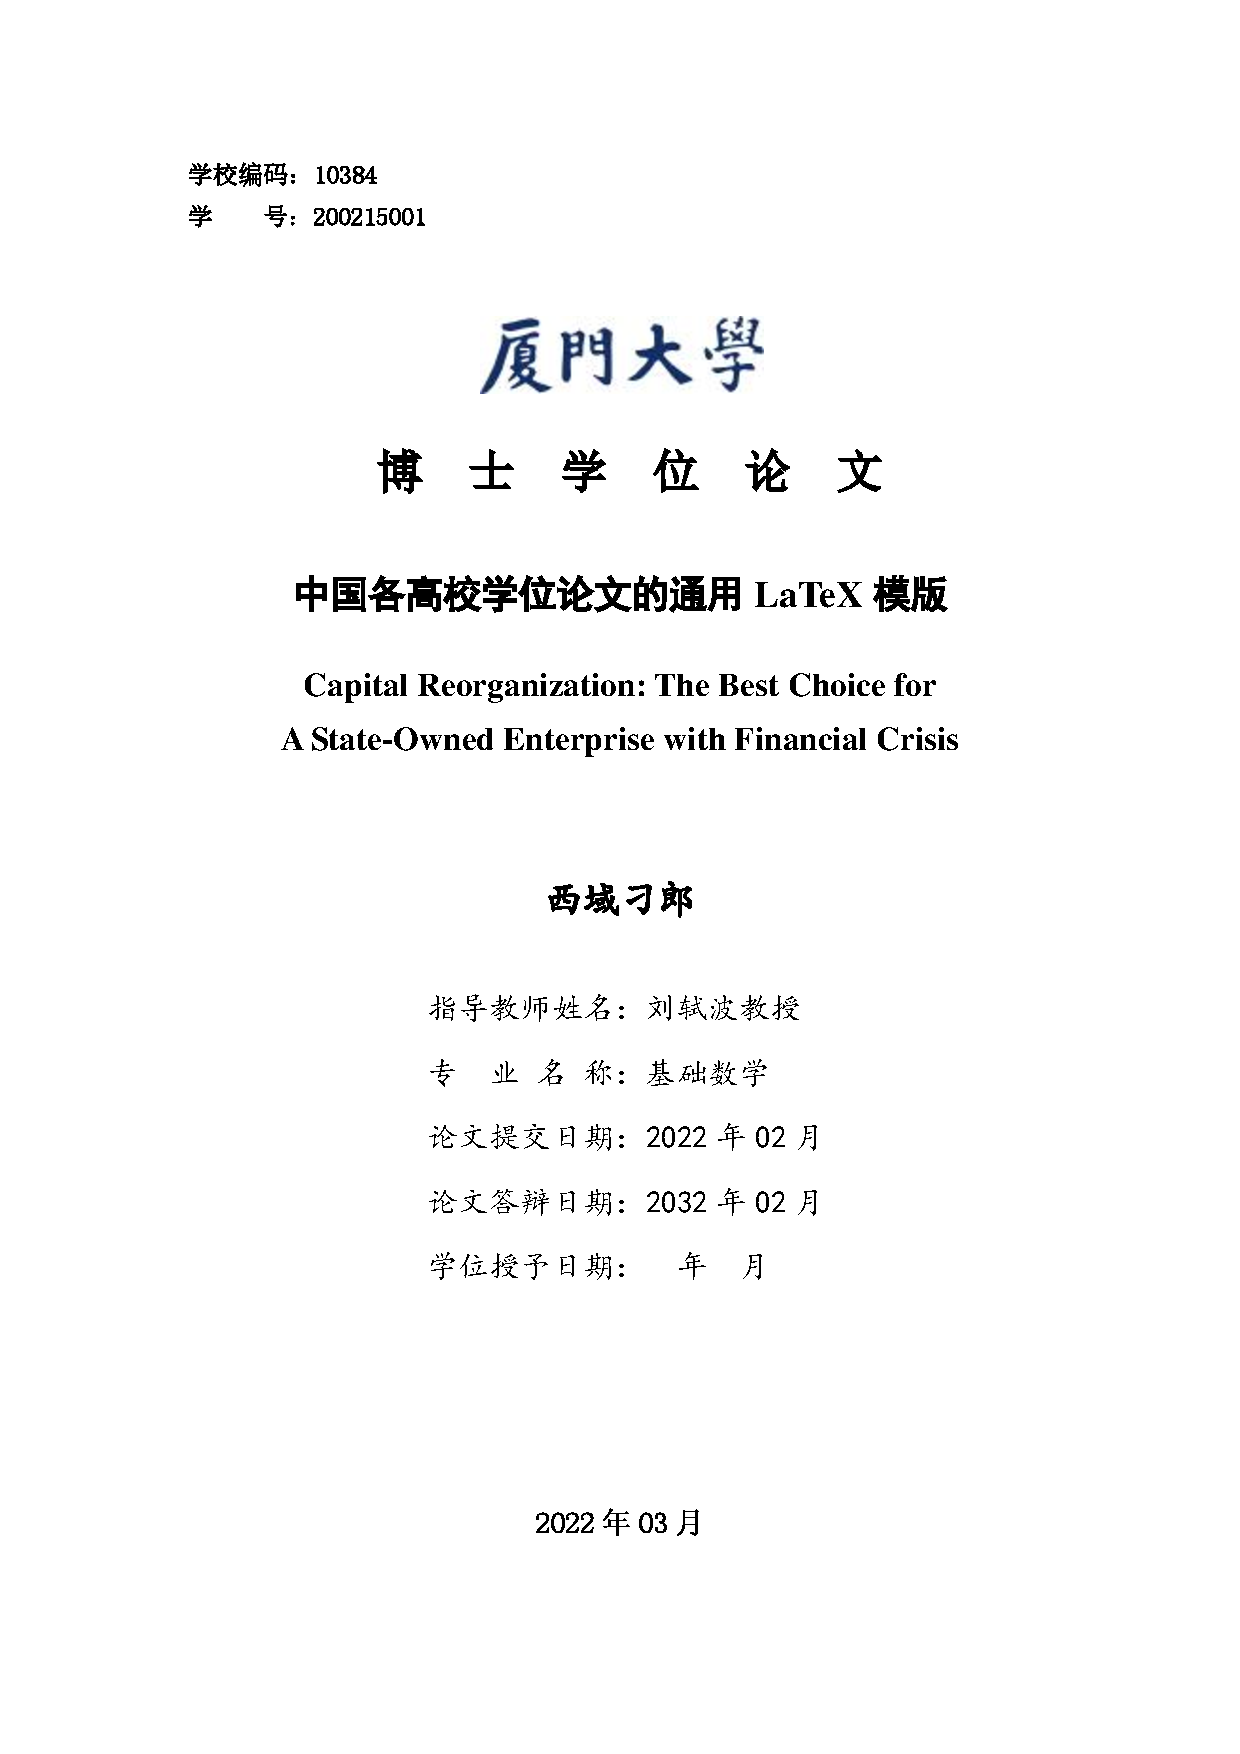
\includegraphics[clip,viewport=88 104 506 767,width=418pt]{cov}\newpage.\newpage

\vspace*{-10pt}
\hspace{-20pt}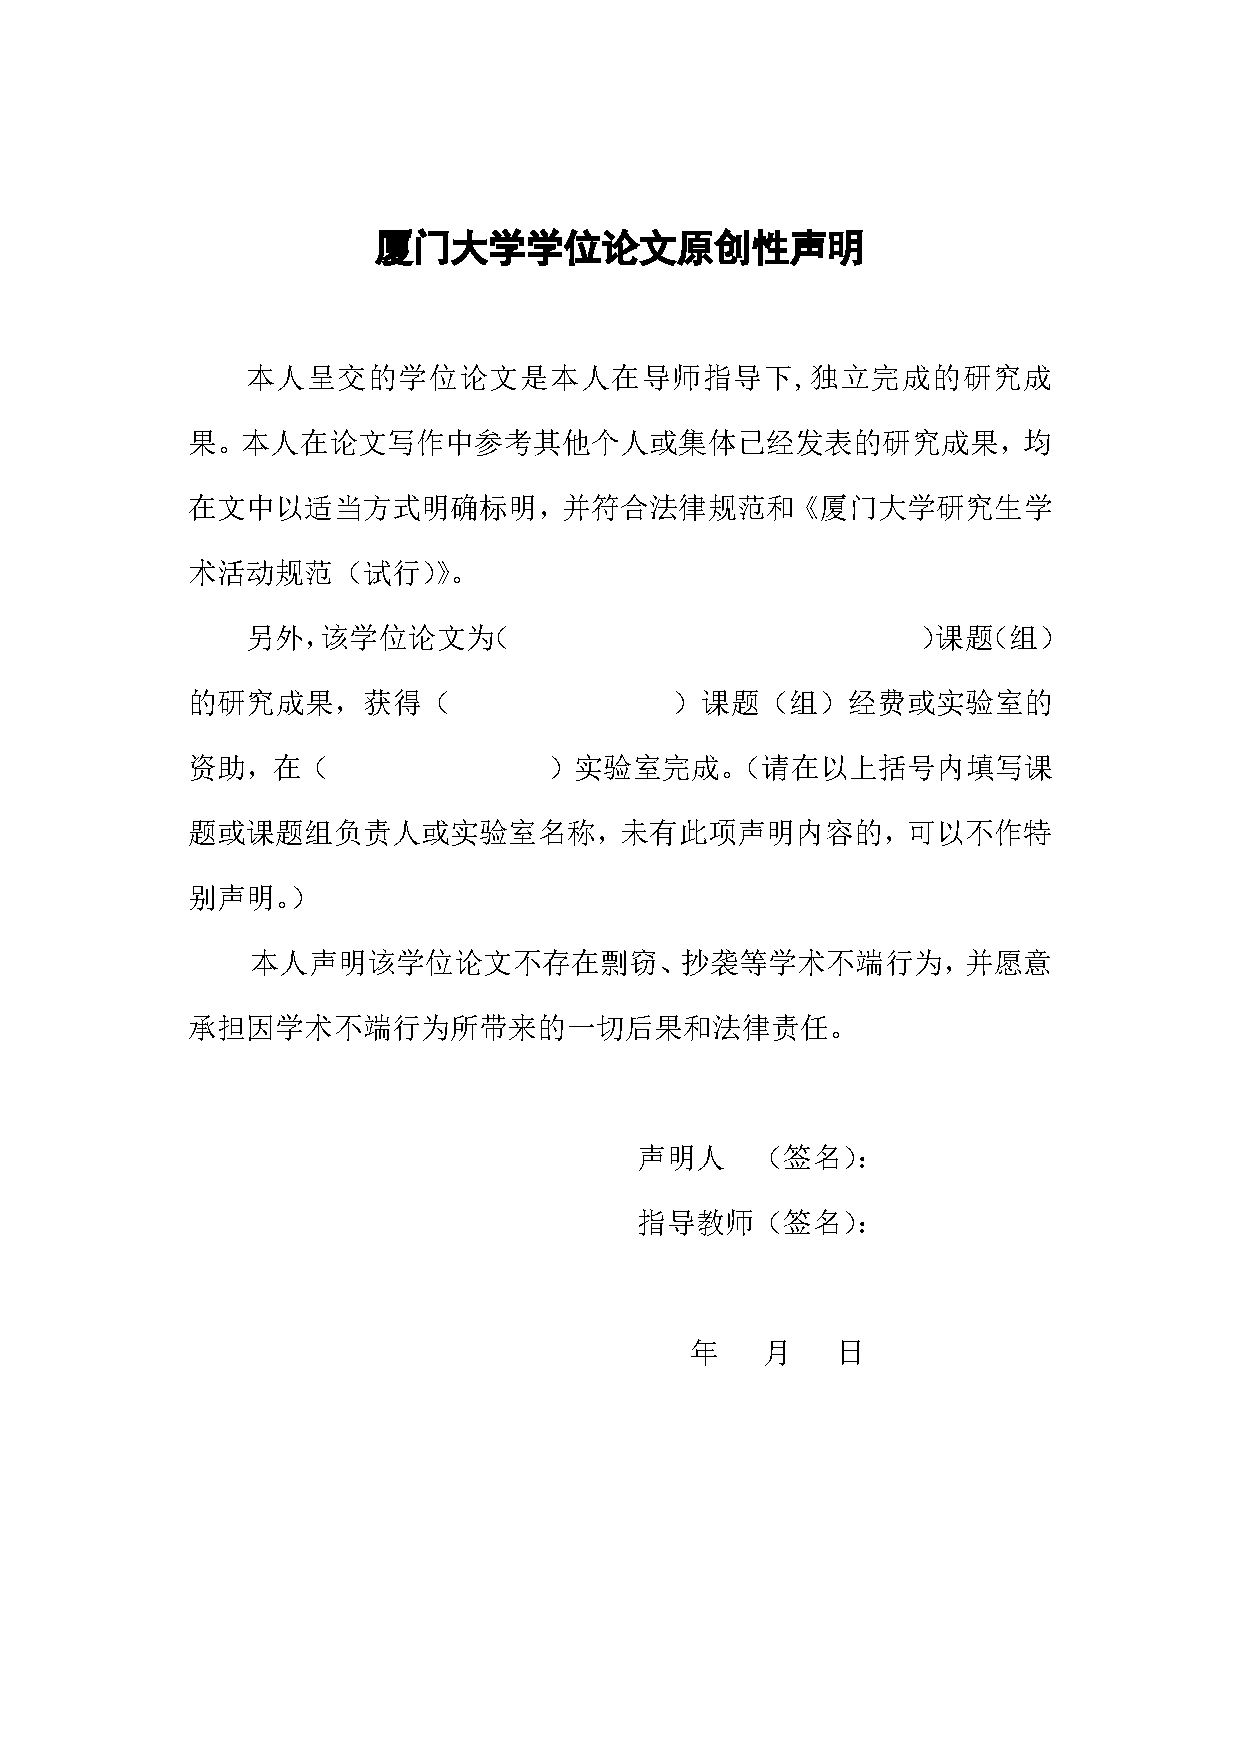
\includegraphics[clip,viewport=88 104 506 767,width=418pt]{org}\newpage.\newpage

\vspace*{-10pt}
\hspace{-20pt}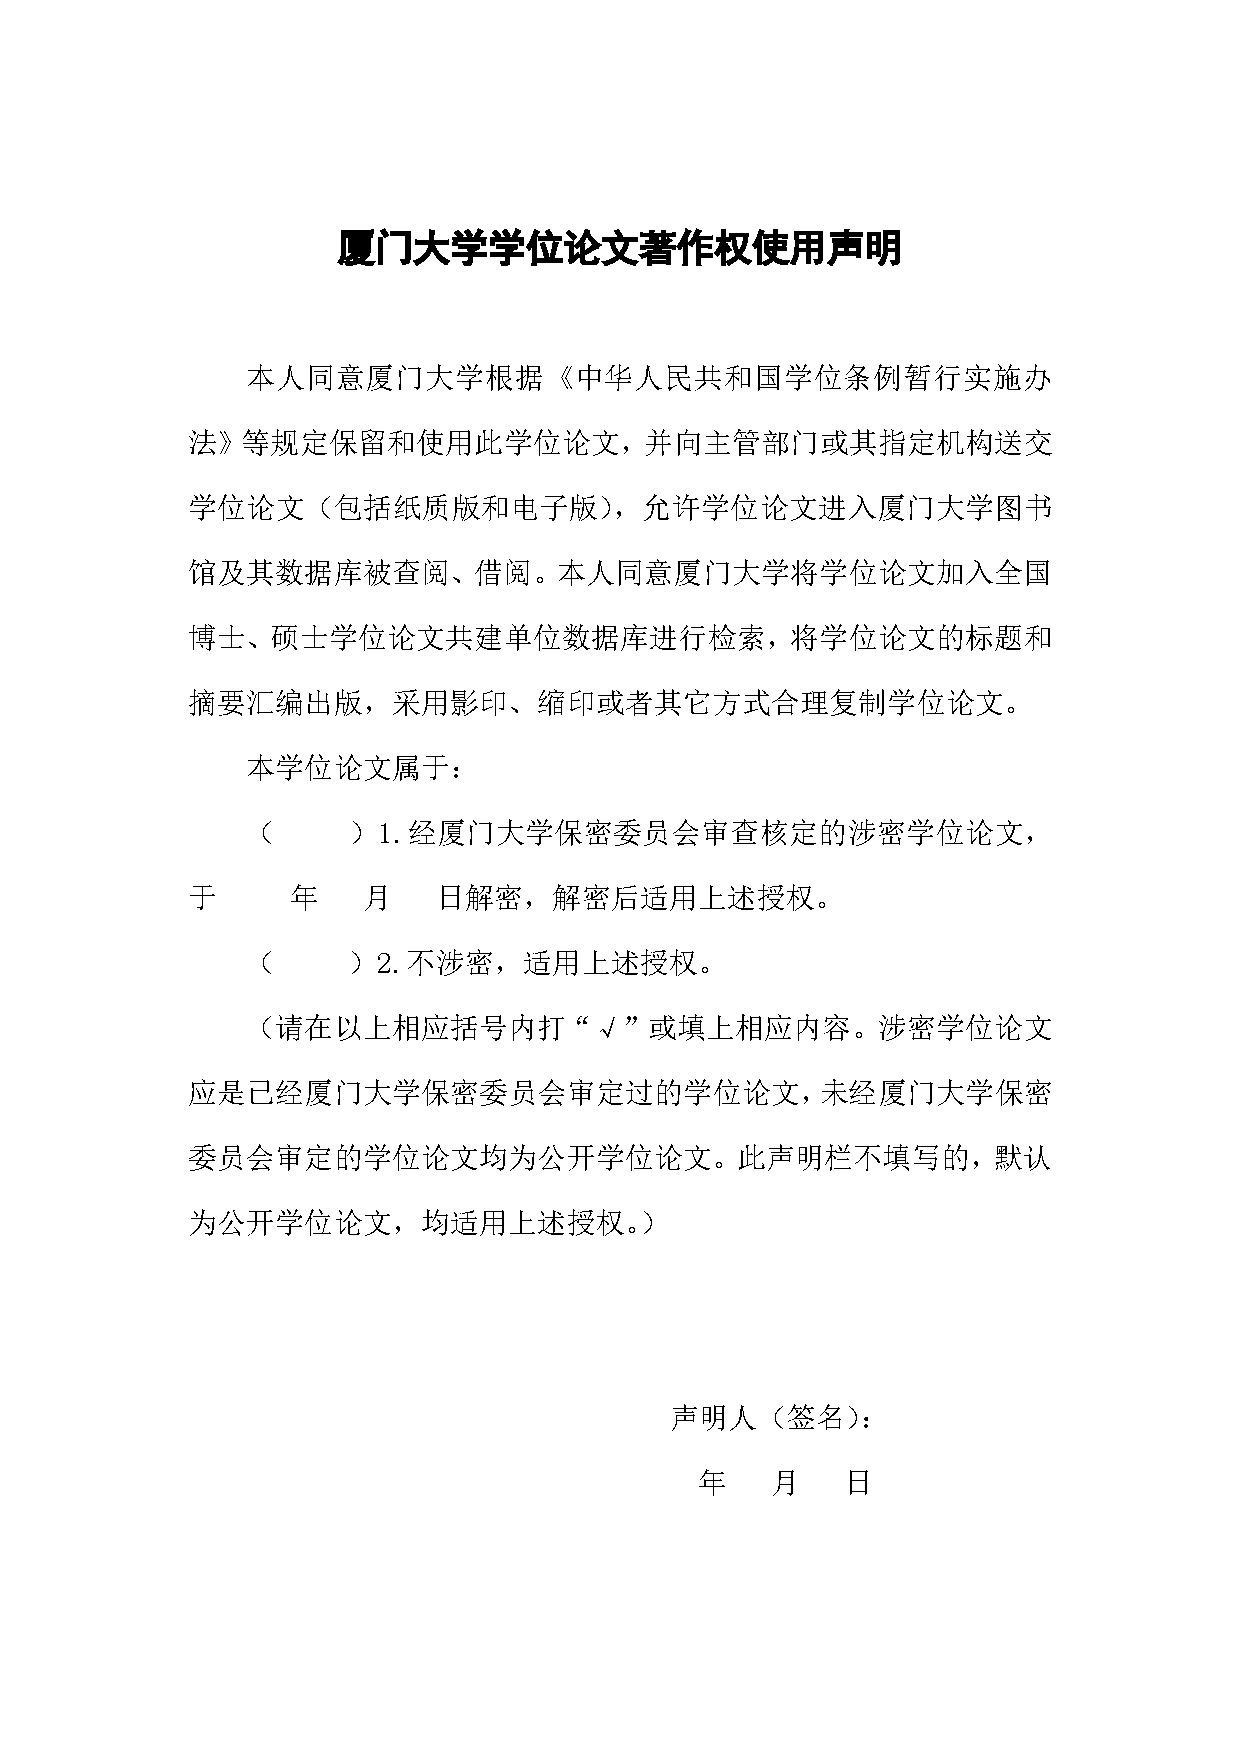
\includegraphics[clip,viewport=88 104 506 767,width=418pt]{use}\newpage.\newpage

%%%%论文内容正式开始

\pagestyle{fancy}\fancyhf{}\fancyhead[LE,RO]{\thepage}

\pagenumbering{roman}


\chapter*{摘要}
\fancyhead[CE]{摘要}\fancyhead[CO]{摘要}
\setcounter{page}{1}
\addcontentsline{toc}{chapter}{\numberline {摘要}}

这是我设计的\emph{厦门大学学位论文}的~\LaTeX{} 模版, 稍作修改可以适用于所有高校. 
本作品的思路是将~Word 格式的封面等转成~PDF, 然后作为图片插入~\TeX{} 中, 这是本人的伟大思想. 此前按此思想制作
的\emph{国家自然科学基金申请书}的~\LaTeX{} 模版, 好评如潮.

其他高校的朋友使用, 可以下载本校的封面、原创声明、使用声明等的~Word 文件, 填写后转成~PDF, 替换掉本模版所附的~\texttt{cov.pdf, org.pdf} 和~\verb|use.pdf|; 也许还需要修改本~\TeX{} 文件第~37, 40, 43 行的~\verb|\includegraphics| 命令中~\verb|viewport| 的参数, 以及~\verb|\hspace| 和~\verb|\vspace| 命令的参数, 使封面等元素显示在页面的适当位置.

\subsection*{使用方法}
\begin{enumerate}
\item 本模版适用于安装了~\CTeX 套装的~Windows 系统, 或已安装了~\verb|ctex| 宏集的任何~\TeX{} 系统, 例如线上的~Overleaf ({\color{blue}\verb|https://www.overleaf.com/|}).
\item 在~cov.doc 中填写论文题目、作者姓名等信息. 存盘后转为~PDF 文件~cov.pdf,用于替换本目录所附的~cov.pdf.
\item 然后,在本~\TeX{} 文件中撰写学位论文的内容(用~\verb|\chap{}| 开始新的一章). 这是为了得到\emph{活动页眉}. 如果本校对页眉有特殊要求, 请用~\verb|\chapter{}| 来开始新的一章并参照~\verb|fancyhdr| 宏包的使用方法修改本~\TeX{} 文件第47, 48行.
\item 按照本校的要求撰写参考文献. 如果使用~BibTeX, 可以选择格式相近的~BST 文件做出参考文献后, 再手动在~\verb|BBL| 文件中修改代码, 得到符合本校要求的文献格式. 此事应该在论文定稿时进行, 以免重新运行~BibTeX 后得重新修改文献格式.

此外, 记得在参考文献中加~\verb|\addcontentsline|命令, 把参考文献加入目录中.
\item 以~\verb|pdflatex| 编译,即可得到学位论文的~PDF 文件.
\end{enumerate}

\hfill 西域刁郎\hspace{17mm}

\hfill \today

\hfill 刘轼波~\TeX{} 排版思想研究中心

\hfill\texttt{\color{blue}{lausb4@gmail.com}}

\chapter*{Abstract}
\fancyhead[CE]{Abstract}\fancyhead[CO]{Abstract}
\addcontentsline{toc}{chapter}{\numberline {Abstract}}

\subsection*{免责声明}

\begin{enumerate}
\item 未经作者允许, 本品禁止用于商业用途.
\item 如需用于商业用途, 请致函~\verb|lausb@gmail.com| 商讨酬金事宜.
\item 使用本作品后果自负, 作者不对任何由此造成的损失承担责任.
\end{enumerate}

\newpage

d

\newpage
%%% End of Abstract

\fancyhead[CE]{\leftmark}\fancyhead[CO]{\S\rightmark}
\tableofcontents


\chap{一元函数积分学}
\pagenumbering{arabic}
\setcounter{page}{1}
\section{原函数和不定积分}

设~$I$ 为区间, $f:I\rightarrow\mathbb{R}$.
我们经常需要寻找函数~$F:I\rightarrow
\mathbb{R}$ 使~$F^{\prime}=f$,
例如已知位移求速度.
这样的函数~$F$ 如果存在,
称其为~$f$ 在~$I$ 上的原函数.

原函数$\Phi$原函数~$\Phi$ 原函数

\begin{exmp}
\label{exp1}设~$f:\left[  a,b\right]  \rightarrow\lbrack0,\infty)$
连续, 求~$f$ 的图像与~$x$ -
轴及直线~$x=a$ 和~$x=b$
所围曲边梯形的\emph{面积}
(称为~$f$ 在~$[a,b]$ 上的面积).
\end{exmp}

\begin{pf}
设~$f$ 在~$[a,x]$ 上的面积为~$A(x)$,
则~$f$ 在~$\left[  x,x+h\right]  $
上的面积为
\[
A(x+h)-A(x)\approx f(x)h\text{.}%
\]
利用~$f$
的连续性可以证明~(练习)
\[
A^{\prime}(x)=\lim_{h\rightarrow0}\frac{A(x+h)-A(x)}{h}=f(x)\text{,}%
\]
因此这~$A$ 就是~$f$
的一个原函数~(满足~$A(a)=0$).
如果求出~$A$,
则欲求面积等于~$A(b)$. 详见\cite{MR3882064,MR2767062}.
\end{pf}

\begin{rem}
注意直到此时我们还没定义什么叫做平面图形的\emph{面积}%
.
\end{rem}

\begin{exmp}
设~$f(x)=x^{2}$, 易见~$F(x)=x^{3}/3$
是其~(满足~$F(0)=0$ 的) 原函数.
因此~$f$ 在~$\left[  0,1\right]  $
上的面积为~$F(1)=1/3$.
\end{exmp}

如果~$F$ 是~$f$ 的原函数,
则对任意~$C\in\mathbb{R}$, $F+C$ 也是~$f$
的原函数; 由~Lagrange
中值定理易见, $f$
的原函数必形如~$F+C$.
函数~$f$
的原函数的\emph{通式}
\begin{equation}
\int f(x)\mathrm{d}x=F(x)+C \label{e1}%
\end{equation}
称为~$f$ 的不定积分.

\subsection{线性性质和分部积分}%


利用导数的性质我们可以写出不定积分的相应性质:%
\begin{align}
&\int\left(  \alpha f+\beta g\right)     =\alpha\int f+\beta\int
g\text{,}\tag{线性性}\\
&\int fg^{\prime}   =fg-\int f^{\prime}g\text{\quad or\quad}\int
fdg=fg+\int gdf\text{.} \tag{分部积分}%
\end{align}


\begin{pf}
[分部积分]因为~$\left(  fg\right)
^{\prime}=f^{\prime}g+fg^{\prime}$,
所以忽略一个可以并入积分记号的常数~$C$
后,%
\[
fg=\int\left(  fg\right)  ^{\prime}=\int\left(  f^{\prime}g+fg^{\prime
}\right)  =\int f^{\prime}g+\int fg^{\prime}\text{.}%
\]

\end{pf}

每一个导数的等式就对应着一个不定积分的等式,
例如\[
\left(  \frac{x^{\alpha+1}}{\alpha+1}\right)  ^{\prime}=x^{\alpha}%
\qquad\longleftrightarrow\qquad\int x^{\alpha}\mathrm{d}x=\frac{x^{\alpha+1}%
}{\alpha+1}+C\text{.}%
\]
所以我们首先要熟悉简单函数的不定积分,
例如\[
\int\cos x\,\mathrm{d}x=\sin x+C\text{.}%
\]
请大家自行写出与课本第~89
页的基本函数导数公式相应的基本函数不定积分公式并熟记.
熟悉这些公式之后,
较复杂的函数的积分可以运用积分的线性性和分部积分公式,
以及我们后面要介绍的换元公式予以解决.
现在,
还可以用一些具有符号计算功能的数学软件~(如~Maple)
用计算机来解决求不定积分的问题.

现在我们来计算一些简单的积分.%
\begin{align*}
\int\frac{x^{2}}{x^{2}+1}\mathrm{d}x  &  =\int\frac{\left(  x^{2}+1\right)
-1}{x^{2}+1}\mathrm{d}x=\int1\,\mathrm{d}x-\int\frac{1}{x^{2}+1}\mathrm{d}x\\
&  =x-\arctan x+C\text{.}\\
\int x\sin x\,\mathrm{d}x  &  =-\int x\left(  \cos x\right)  ^{\prime
}\,\mathrm{d}x=-x\cos x+\int\cos x\cdot\left(  x\right)  ^{\prime}%
\mathrm{d}x\\
&  =-x\cos x+\int\cos x\,\mathrm{d}x=-x\cos x+\sin x+C\text{.}%
\end{align*}
习惯上我们把上面第~2
个积分的计算过程写成\[
\int x\sin x\,\mathrm{d}x=\int x\,\mathrm{d}\left(  -\cos x\right)  =-x\cos
x+\int\cos x\,\mathrm{d}x\text{,}%
\]
俗称让~$\sin x$
进入\emph{微分号}.
用分部积分法计算乘积的积分,
谁该优先进入微分号呢?
经验表明按照\emph{反对幂三指}%
的相反顺序是合适的.%
\begin{align*}
\int x^{3}e^{x}\,\mathrm{d}x  &  =\int x^{3}\mathrm{d}e^{x}=x^{3}e^{x}-\int
e^{x}\mathrm{d}x^{3}=x^{3}e^{x}-3\int x^{2}e^{x}\,\mathrm{d}x=\cdots\text{.}\\
\int x\ln^{2}x\,\mathrm{d}x  &  =\int\ln^{2}x\,\mathrm{d}\left(  \frac{x^{2}%
}{2}\right)  =\frac{x^{2}}{2}\ln^{2}x-\int\frac{x^{2}}{2}\mathrm{d}\left(
\ln^{2}x\right) \\
&  =\frac{x^{2}}{2}-\int\frac{x^{2}}{2}\cdot2\frac{\ln x}{x}\,\mathrm{d}%
x=\frac{x^{2}}{2}-\int x\ln x\,\mathrm{d}x=\cdots\text{.}%
\end{align*}
以上两个例子都是按照上述经验来计算的.
对于第二个例子, 让~$\ln^{2}x$
进入微分号,
就需要找一个导数为~$\ln
^{2}x$ 的函数,
这也是难以办到的.%
\begin{align*}
\int e^{x}\sin x\,\mathrm{d}x  &  =\int\sin x\,\mathrm{d}e^{x}=e^{x}\sin
x-\int e^{x}\mathrm{d}\left(  \sin x\right) \\
&  =e^{x}\sin x-\int e^{x}\cos x\,\mathrm{d}x=e^{x}\sin x-\int\cos
x\,\mathrm{d}e^{x}\\
&  =e^{x}\sin x-\left(  e^{x}\cos x-\int e^{x}\,\mathrm{d}(\cos x)\right) \\
&  =e^{x}\left(  \sin x-\cos x\right)  -\int e^{x}\sin x\,\mathrm{d}x\text{.}%
\end{align*}
分部积分后等式右边又出现了欲算的积分,
于是视其为未知元解方程得\[
\int e^{x}\sin x\,\mathrm{d}x=\frac{e^{x}\left(  \sin x-\cos x\right)  }%
{2}+C\text{.}%
\]
这个例子也可以让~$\sin x$
进入微分号来计算.
其实,
指数函数和三角函数有密切的关系,
它们有很相似的基本性质.

\subsection{换元积分法}

\begin{enumerate}
\item 如果~$F$ 是~$f$ 的原函数,
则~$F\circ\varphi$ 是~$\left(  f\circ\varphi\right)
\varphi^{\prime}$ 的原函数, 即\begin{equation}
\int f(\varphi(x))\varphi^{\prime}(x)\,\mathrm{d}x=F(\varphi(x))+C=\left(
\int f(u)\,\mathrm{d}u\right)  _{u=\varphi(x)}\text{.}
\tag{凑微分法}%
\end{equation}


\item 设~$\varphi$ 有反函数~$\psi$.
如果~$\Phi$ 是~$\left(  f\circ\varphi\right)  \varphi
^{\prime}$ 的原函数, 则~$\Phi\circ\psi$
是~$f$ 的原函数, 即\begin{equation}
\int f(u)\,\mathrm{d}u=\Phi(\psi(u))+C=\left(  \int f(\varphi(x))\varphi
^{\prime}(x)\,\mathrm{d}x\right)  _{x=\psi(u)}\text{.}%
\tag{代入法}%
\end{equation}

\end{enumerate}

\begin{rem}
以上两个换元法的等式,
需要证明的都是第一个等号,
第二个等号不过是不定积分的定义而已.
\end{rem}

\begin{pf}
利用链法则和反函数求导法则直接计算\begin{align*}
\left(  \Phi\circ\psi\right)  ^{\prime}(u) &  =\Phi^{\prime}(\psi
(u))\psi^{\prime}(u)\\
&  =\left[  f(\varphi(x))\varphi^{\prime}(x)\right]  _{x=\psi(u)}\cdot\frac
{1}{\left[  \varphi^{\prime}(x)\right]  _{x=\psi(u)}}\\
&  =f(\varphi(\psi(u)))=f(u)\text{.}%
\end{align*}

\end{pf}

\begin{rem}
形式上看, 在~(1) 中,
我们视~$u^{\prime}(x)\mathrm{d}x$ 为~$u$
的微分~$\mathrm{d}u$,
转化为计算以~$u$
为变量的另一个积分,
所以称为凑微分法; 在~(2)
中, 我们把~$u=\varphi(x)$
代入被积表达式~$f(u)\mathrm{d}u$,
转化为计算以~$x$
为变量的积分, 所以称为代入法.
\end{rem}

例如用凑微分法可得\begin{align}
I  &  =\int\sqrt{\sin x}\cos x\,\mathrm{d}x=\int\sqrt{\sin x}\,\mathrm{d}(\sin
x)\tag{$u=\sin x$}\\
&  =\int\sqrt{u}\,\mathrm{d}u=\frac{2}{3}u^{3/2}+C=\frac{2}{3}\left(  \sin
x\right)  ^{3/2}+C\text{.}\nonumber
\end{align}


\begin{exmp}
计算~$I=\displaystyle\int\frac{\mathrm{d}x}{x\sqrt{1+x^{2}}}$.

用凑微分法,%
\begin{align}
I  &  =\int\frac{\mathrm{d}x}{x^{2}\sqrt{1+\left(  \frac{1}{x}\right)  ^{2}}%
}=-\int\frac{1}{\sqrt{1+\left(  \frac{1}{x}\right)  ^{2}}}\mathrm{d}\left(
\frac{1}{x}\right) \tag{$u=\frac{1}{x}$}\\
&  =-\int\frac{\mathrm{d}u}{\sqrt{1+u^{2}}}=-\ln\left\vert u+\sqrt{1+u^{2}%
}\right\vert +C\tag{P.89 例~4.1.11}\\
&  =\ln\frac{\left\vert x\right\vert }{1+\sqrt{1+x^{2}}}+C\text{.}\nonumber
\end{align}
或者作代换~$x=\tan
t$ ($|t|<\pi/2$), $\mathrm{d}x=\sec^{2}t\,\mathrm{d}t$,
于是~(直角三角形计算)%
\begin{equation}
\cos t=\frac{1}{\sqrt{1+x^{2}}}\text{.}\label{ru}%
\end{equation}
由代入法,%
\begin{align}
\hspace{25mm}I &  =\int\frac{\sec^{2}t\,\mathrm{d}t}{\tan t\sec t}=\int%
\frac{\mathrm{d}t}{\sin t}=\int\frac{\sin t\,\mathrm{d}t}{1-\cos^{2}t}%
\tag{$u=\cos t$}\\
&  =-\int\frac{\mathrm{d}u}{1-u^{2}}=\frac{1}{2}\ln\left\vert \frac{u-1}%
{u+1}\right\vert +C\nonumber\\
&  =\frac{1}{2}\ln\left\vert \frac{\cos t-1}{\cos t+1}\right\vert +C=\frac
{1}{2}\ln\left\vert \frac{1-\frac{1}{\sqrt{1+x^{2}}}}{1+\frac{1}{\sqrt
{1+x^{2}}}}\right\vert +C\label{xc}\\
&  =\ln\frac{\left\vert x\right\vert }{1+\sqrt{1+x^{2}}}+C\text{.}\nonumber
\end{align}

\end{exmp}

\begin{rem}
以上计算的~(\ref{xc}) 中,
我们直接利用~(\ref{ru}%
) 整体地将~$\cos t$ 用~$x$ 表示,
而不是死板地用换元函数的反函数~$t=\arctan
x$ 计算:%
\[
\frac{1}{2}\ln\left\vert \frac{\cos t-1}{\cos t+1}\right\vert +C=\frac{1}%
{2}\ln\left\vert \frac{\cos\arctan x-1}{\cos\arctan t+1}\right\vert +C\text{.}%
\]

\end{rem}

三角代换是计算含~$\sqrt
{ax^{2}+bx+c}$
的积分的常用方法.
例如设~$x=a\sin t$ ($\left\vert t\right\vert \leq\pi/2$);
$\mathrm{d}x=a\cos t\,\mathrm{d}t$, 于是\begin{align}
I  &  =\int\sqrt{a^{2}-x^{2}}\mathrm{d}x=\int a\cos t\cdot a\cos
t\,\mathrm{d}t=\int a^{2}\cos^{2}t\,\mathrm{d}t\tag{$a>0$}\\
&  =a^{2}\int\frac{1+\cos2t}{2}\mathrm{d}t=a^{2}\left(  \frac{t}{2}+\frac
{1}{4}\sin2t+C^{\prime}\right) \nonumber\\
&  =a^{2}\left(  \frac{t}{2}+\frac{1}{2}\sin t\cos t+C^{\prime}\right)
\nonumber\\
&  =a^{2}\left(  \frac{1}{2}\arcsin\frac{x}{a}+\frac{1}{2}\frac{x}{a}%
\sqrt{1-\left(  \frac{x}{a}\right)  ^{2}}+C^{\prime}\right) \nonumber\\
&  =\frac{a^{2}}{2}\arcsin\frac{x}{a}+\frac{x\sqrt{a^{2}-x^{2}}}{2}%
+C\text{.}\nonumber
\end{align}
但是这个积分用分部积分法也可以计算:%
\begin{align*}
I  &  =\int\sqrt{a^{2}-x^{2}}\mathrm{d}x=x\sqrt{a^{2}-x^{2}}-\int
x\,\mathrm{d}\sqrt{a^{2}-x^{2}}\\
&  =x\sqrt{a^{2}-x^{2}}-\int x\cdot\frac{-x}{\sqrt{a^{2}-x^{2}}}\mathrm{d}x\\
&  =x\sqrt{a^{2}-x^{2}}-\int\frac{\left(  a^{2}-x^{2}\right)  -a^{2}}%
{\sqrt{a^{2}-x^{2}}}\mathrm{d}x\\
&  =x\sqrt{a^{2}-x^{2}}-I+a^{2}\int\frac{1}{\sqrt{a^{2}-x^{2}}}\mathrm{d}x\\
&  =x\sqrt{a^{2}-x^{2}}-I+a^{2}\arcsin\frac{x}{a}+C^{\prime}\text{.}%
\end{align*}
于是\[
I=\frac{x\sqrt{a^{2}-x^{2}}}{2}+\frac{a^{2}}{2}\arcsin\frac{x}{a}+C\text{.}%
\]


\section{曲边梯形的面积与定积分的定义}%


我们换一种方法来考虑例~\ref{exp1}%
. 我们称~$\left[  a,b\right]  $ 的含~$a,b$
的有限子集~$P=\left\{  x_{i}\right\}  _{i=0}%
^{n}$ 为~$\left[  a,b\right]  $ 的划分,
不妨设\[
a=x_{0}<\cdots<x_{n}=b\text{.}%
\]
取~$\left[  a,b\right]  $ 的划分~$P=\left\{
x_{i}\right\}  _{i=0}^{n}$, 对~$i\in\overline{n}$ 取~$\xi_{i}%
\in\left[  x_{i-1},x_{i}\right]  $. $f$ 在~$\left[  x_{i-1}%
,x_{i}\right]  $
上的面积约等于~$f(\xi_{i})\Delta
x_{i}$, 这里~$\Delta x_{i}=x_{i}-x_{i-1}$.
于是欲求面积的近似值~(依赖于划分~$P$
及样点组~$\{\xi_{i}\}_{i=1}^{n}$)
\[
A(P,\xi)=\sum_{i=1}^{n}f(\xi_{i})\Delta x_{i}\text{.}%
\]
直观上, 当划分~$P$
越来越精细, 即\[
\left\vert P\right\vert =\max_{i\in\overline{n}}\Delta x_{i}\rightarrow0
\]
时, $A(P,\xi)$
应该趋于曲边梯形的面积~$A$
. 记此极限为~$\int_{a}^{b}f$,
称为~$f$ 在~$\left[  a,b\right]  $
的定积分, 则\[
A=\int_{a}^{b}f(x)\,\mathrm{d}x\text{.}%
\]
再看一个例子.
设一变密度细棒占据区间~$\left[
a,b\right]  $, 设~$x$
处的线密度是~$\rho(x)$,
我们来求其质量~$m$.
作~$\left[  a,b\right]  $ 的划分~$P=\left\{
x_{i}\right\}  _{i=0}^{n}$ 将细棒分成~$n$
段, 取~$\xi_{i}\in\left[  x_{i-1},x_{i}\right]  $.
则第~$i$
段的质量近似于~$\rho(\xi_{i})\Delta
x_{i}$, 因此\[
m\approx\sum_{i=1}^{n}\rho(\xi_{i})\Delta x_{i}\text{.}%
\]
可以相信,
当划分越来越精细,
即~$\left\vert P\right\vert \rightarrow0$ 时,
上式右端越来越接近细棒的实际质量~$m$%
. 于是\[
m=\lim_{\left\vert P\right\vert \rightarrow0}\sum_{i=1}^{n}\rho(\xi_{i})\Delta
x_{i}=\int_{a}^{b}\rho(x)\,\mathrm{d}x\text{.}%
\]


很多实际问题中都需要计算形如~${\textstyle\sum
\limits_{i=1}^{n}} f(\xi_{i})\Delta x_{i}$
的和在~$\left\vert P\right\vert \rightarrow0$
时的极限, 因此我们引入如下定义.

\begin{defn}
设~$f:\left[  a,b\right]  \rightarrow\mathbb{R}$, $I\in\mathbb{R}$.
若对~$\forall\varepsilon>0$, $\exists\delta>0$,
对于~$\left[  a,b\right]  $
的任何划分~$P=\left\{  x_{i}\right\}  _{i=0}%
^{n}$, 只要~$\left\vert P\right\vert <\delta$, 对~$\forall
\xi_{i}\in\left[  x_{i-1},x_{i}\right]  $ 总有\[
\left\vert \sum_{i=1}^{n}f(\xi_{i})\Delta x_{i}-I\right\vert <\varepsilon
\text{,}%
\]
就称~$f$ 在~$\left[  a,b\right]  $ 可积,
称~$I$ 为~$f$ 在~$\left[  a,b\right]  $
的定积分, 记为\[
I=\int_{a}^{b}f(x)\,\mathrm{d}x\text{.}%
\]

\end{defn}

\begin{rem}
我们可以不太严格地说定积分是~Riemann
和的极限\[
\int_{a}^{b}f(x)\,\mathrm{d}x=\lim_{\left\vert P\right\vert \rightarrow0}%
\sum_{i=1}^{n}f(\xi_{i})\Delta x_{i}\text{.}%
\]
需要注意的是,
右端的极限与以前学习的函数极限是不同的,
给定了极限变量~$\left\vert
P\right\vert $ 的值,
被取极限的和式~(称为~Riemann
和) 并不确定,
它还依赖于~$P$
以及\emph{样点组}~$\left\{  \xi_{i}\right\}
_{i=1}^{n}$ 的选择.
\end{rem}


%%%% 参考文献
%\bibliographystyle{siam}
%\bibliography{ref}

\begin{thebibliography}{Liu10}
\addcontentsline{toc}{chapter}{\numberline {参考文献}}


\bibitem[Liu10]{MR2767062}
\textsc{S.~Liu}, \href{https://doi.org/10.4169/000298910X523425}{On the
  regularity of operators near a regular operator}, Amer. Math. Monthly,
  117(2010) 927--928.

\bibitem[LL18]{MR3882064}
\textsc{P.~Liu}, \textsc{S.~Liu},
  \href{https://doi.org/10.1080/00029890.2018.1521241}{On the surjectivity of
  smooth maps into {E}uclidean spaces and the fundamental theorem of algebra},
  Amer. Math. Monthly, 125(2018) 941--943.

\end{thebibliography}


\end{document}